\section{Introduction to Control Rods}

\subsection{Functions}
Control rods are essential for \textbf{modulating reactivity}, serving the following functions:
\begin{itemize}
    \item Compensating for excess reactivity due to fuel consumption or thermal feedback
    \item Regulating the neutron population
    \item Providing a safety margin for shutdown
    \item Assisting in reactor startup
\end{itemize}

\subsection{Physical Behavior}
Control rods function as \textbf{neutron absorbers} by altering the absorption component of $K_{eff}$:
\begin{equation}
    K_{eff} = \frac{Production}{Absorption + Leakages} = \frac{\int \int \nu \Sigma_f \phi dV dE}{\int \int _{fuel} \Sigma_a \phi dV dE + \dot{L}}
\end{equation}

\subsection{Effects}
The insertion of a control rod modifies the neutron flux distribution. Its effectiveness depends on its absorption capability and the neutron flux in its vicinity.

\begin{figure}[h]
    \centering
    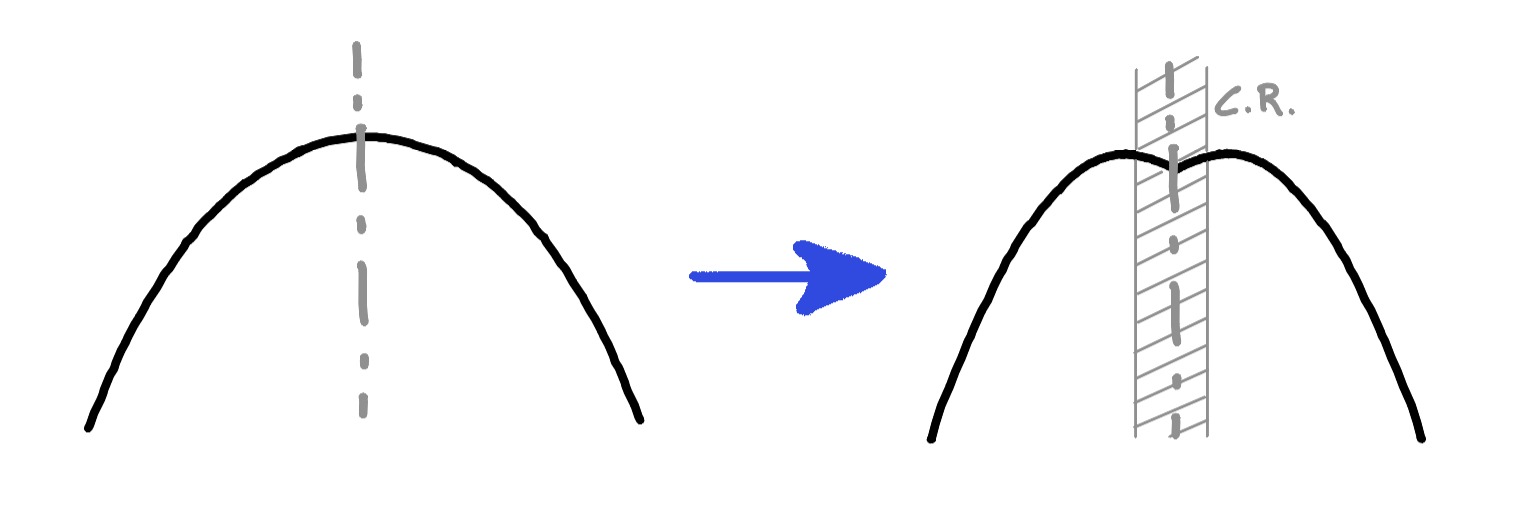
\includegraphics[width=0.75\linewidth]{CR_3.png}
    \caption{Flux before and after control rod insertion}
\end{figure}

\textbf{Shadowing effect}: The position of one control rod can impact the effectiveness of another.

\subsection{Design}
\begin{wrapfigure}{r}{0.3\textwidth}
    \begin{tcolorbox}[boxstyle, title=DESIGN STEPS]
        1. Materials \\
        2. Geometry \\
        3. Quantity
    \end{tcolorbox}
\end{wrapfigure} 
The material selection is critical, requiring a substance with high absorption capabilities. For example, $B^{10}$ primarily undergoes (n,$\alpha$) reactions, while Gadolinium is more likely to produce (n,$\gamma$) reactions, which raises radiological safety concerns. \\
Following material selection, the rod geometry is typically constrained by overall design parameters. \\
Finally, the required number of rods, or equivalently the $pcm$, is determined by the need to compensate for excess reactivity at the start of the fuel cycle and provide an adequate shutdown margin.

\begin{figure}[h]
    \centering
    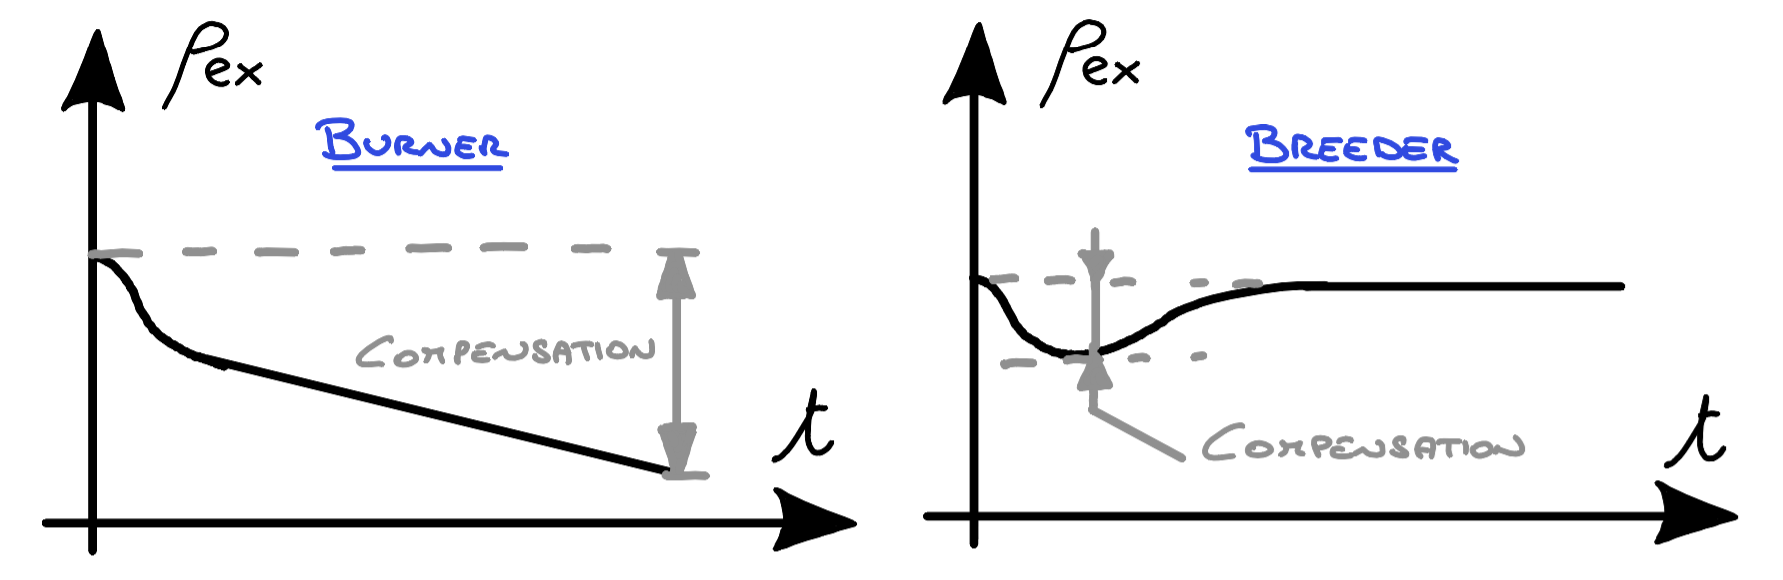
\includegraphics[width=0.75\linewidth]{CR_1.png}
    \caption{Reactivity worth needed for fuel consumption compensation is generally lower in breeder reactors compared to burner reactors.}
\end{figure}
